\documentclass[11pt]{article}\usepackage[]{graphicx}\usepackage[]{xcolor}
% maxwidth is the original width if it is less than linewidth
% otherwise use linewidth (to make sure the graphics do not exceed the margin)
\makeatletter
\def\maxwidth{ %
  \ifdim\Gin@nat@width>\linewidth
    \linewidth
  \else
    \Gin@nat@width
  \fi
}
\makeatother

\definecolor{fgcolor}{rgb}{0.345, 0.345, 0.345}
\newcommand{\hlnum}[1]{\textcolor[rgb]{0.686,0.059,0.569}{#1}}%
\newcommand{\hlsng}[1]{\textcolor[rgb]{0.192,0.494,0.8}{#1}}%
\newcommand{\hlcom}[1]{\textcolor[rgb]{0.678,0.584,0.686}{\textit{#1}}}%
\newcommand{\hlopt}[1]{\textcolor[rgb]{0,0,0}{#1}}%
\newcommand{\hldef}[1]{\textcolor[rgb]{0.345,0.345,0.345}{#1}}%
\newcommand{\hlkwa}[1]{\textcolor[rgb]{0.161,0.373,0.58}{\textbf{#1}}}%
\newcommand{\hlkwb}[1]{\textcolor[rgb]{0.69,0.353,0.396}{#1}}%
\newcommand{\hlkwc}[1]{\textcolor[rgb]{0.333,0.667,0.333}{#1}}%
\newcommand{\hlkwd}[1]{\textcolor[rgb]{0.737,0.353,0.396}{\textbf{#1}}}%
\let\hlipl\hlkwb

\usepackage{framed}
\makeatletter
\newenvironment{kframe}{%
 \def\at@end@of@kframe{}%
 \ifinner\ifhmode%
  \def\at@end@of@kframe{\end{minipage}}%
  \begin{minipage}{\columnwidth}%
 \fi\fi%
 \def\FrameCommand##1{\hskip\@totalleftmargin \hskip-\fboxsep
 \colorbox{shadecolor}{##1}\hskip-\fboxsep
     % There is no \\@totalrightmargin, so:
     \hskip-\linewidth \hskip-\@totalleftmargin \hskip\columnwidth}%
 \MakeFramed {\advance\hsize-\width
   \@totalleftmargin\z@ \linewidth\hsize
   \@setminipage}}%
 {\par\unskip\endMakeFramed%
 \at@end@of@kframe}
\makeatother

\definecolor{shadecolor}{rgb}{.97, .97, .97}
\definecolor{messagecolor}{rgb}{0, 0, 0}
\definecolor{warningcolor}{rgb}{1, 0, 1}
\definecolor{errorcolor}{rgb}{1, 0, 0}
\newenvironment{knitrout}{}{} % an empty environment to be redefined in TeX

\usepackage{alltt}
\usepackage{amsmath,amssymb,amsthm}
\title{ISCD Homework 5}
\author{
\begin{tabular}{c}
Anurag Bhunia (bmat2508@isibang.ac.in)\\[0.6em]
\end{tabular}
}
\date{}
%%%%%%%%%%%%%%%Setting Page Sizes %%%%%%%%%%%%
\setlength{\parindent}{0in}
\setlength{\parskip}{\baselineskip}
\setlength{\textheight}{9in}
\setlength{\textwidth}{6.3in}
\setlength{\topmargin}{-0.6in}
\setlength{\evensidemargin}{-.5in}
\setlength{\oddsidemargin}{0in}
%%%%%%%%%%%%%%%%%%%%%%%%%%%%%%%%%%%%%%%%%%%
%%%%%%%%%%%%To make R commands appear in different Color%%%%%%%%%%
\usepackage{color}
\usepackage{fancyvrb} % Verbatim
\usepackage{color}
\definecolor{codecolor}{RGB}{114,12,112}
\DefineVerbatimEnvironment{Sinput}{Verbatim}{formatcom=\color{codecolor}}
\DefineVerbatimEnvironment{Soutput}{Verbatim}{formatcom=\color{codecolor}}
\DefineVerbatimEnvironment{Scode}{Verbatim}{formatcom=\color{codecolor}}
\DefineVerbatimEnvironment{Sin}{Verbatim}{formatcom=\color{codecolor}}
\DefineVerbatimEnvironment{Sout}{Verbatim}{formatcom=\color{codecolor}}
%%%%%%%%%%%%%%%%%%%%%%%%%%%%%%%%%%%%%%%%%%%%%%%%%%%%%%%%%%%%%%%%

\IfFileExists{upquote.sty}{\usepackage{upquote}}{}
\begin{document}
\maketitle
1. Given that $X_1,\dots,X_n$ are i.i.d $\mathcal{N}(\mu,\sigma^2)$.
The joint density function of the sample is
\[
f(x_1,\ldots,x_n \mid \mu,\sigma^2)
= \prod_{i=1}^n \frac{1}{\sqrt{2\pi\sigma^2}}
\exp\!\left(-\frac{(x_i-\mu)^2}{2\sigma^2}\right)
\]

This product is the likelihood function
\[
L(\mu,\sigma^2)
= (2\pi\sigma^2)^{-n/2}
\exp\!\left(-\frac{1}{2\sigma^2}\sum_{i=1}^n (x_i-\mu)^2\right)
\]

Taking logarithms gives the log-likelihood
\[
\ell(\mu,\sigma^2)
= -\frac{n}{2}\log(2\pi)
-\frac{n}{2}\log(\sigma^2)
-\frac{1}{2\sigma^2}\sum_{i=1}^n (x_i-\mu)^2
\]

To find the maximum likelihood estimator of $\mu$, we differentiate with respect to $\mu$
\[
\frac{\partial \ell}{\partial \mu}
= \frac{1}{\sigma^2}\sum_{i=1}^n (x_i-\mu)
\]

Setting this derivative equal to zero gives
\[
\sum_{i=1}^n (x_i-\mu)=0
\]

Solving for $\mu$ yields
\[
\hat{\mu}=\frac{1}{n}\sum_{i=1}^n x_i
\]

Next, we differentiate the log-likelihood with respect to $\sigma^2$
\[
\frac{\partial \ell}{\partial \sigma^2}
= -\frac{n}{2\sigma^2}
+\frac{1}{2(\sigma^2)^2}\sum_{i=1}^n (x_i-\mu)^2
\]

Setting this equal to zero gives
\[
-\frac{n}{2\sigma^2}
+\frac{1}{2(\sigma^2)^2}\sum_{i=1}^n (x_i-\mu)^2=0
\]

Multiplying both sides by $2(\sigma^2)^2$ yields
\[
-n\sigma^2+\sum_{i=1}^n (x_i-\mu)^2=0
\]

Solving for $\sigma^2$ gives
\[
\hat{\sigma}^2=\frac{1}{n}\sum_{i=1}^n (x_i-\mu)^2
\]

Substituting $\hat{\mu}$ into this expression yields the maximum likelihood estimator
\[
\hat{\sigma}^2=\frac{1}{n}\sum_{i=1}^n (x_i-\bar{x})^2
\]
Thus $\hat{\mu}$ is the sample mean and $\hat{\sigma^2}$ is the sample variance.\\ \\ \\
2. We are given that $X_1,\dots,X_n$ are i.i.d Pois($\lambda$).
The probability mass function of a Poisson random variable is
\[
\mathbb{P}(X=x)=\frac{e^{-\lambda}\lambda^x}{x!}, \quad x=0,1,2,\ldots
\]

The joint probability mass function of the sample is
\[
f(x_1,\ldots,x_n \mid \lambda)
= \prod_{i=1}^n \frac{e^{-\lambda}\lambda^{x_i}}{x_i!}
\]

This product is the likelihood function
\[
L(\lambda)
= e^{-n\lambda}\lambda^{\sum_{i=1}^n x_i}\prod_{i=1}^n \frac{1}{x_i!}
\]

Taking logarithms gives the log-likelihood
\[
\ell(\lambda)
= -n\lambda + \left(\sum_{i=1}^n x_i\right)\log\lambda
- \sum_{i=1}^n \log(x_i!)
\]

To find the maximum likelihood estimator, we differentiate with respect to $\lambda$
\[
\frac{d\ell}{d\lambda}
= -n + \frac{1}{\lambda}\sum_{i=1}^n x_i
\]

Setting this derivative equal to zero gives
\[
-n + \frac{1}{\lambda}\sum_{i=1}^n x_i = 0
\]

Solving for $\lambda$ yields
\[
\hat{\lambda} = \frac{1}{n}\sum_{i=1}^n x_i
\]

Thus the maximum likelihood estimator of $\lambda$ is the sample mean
\[
\hat{\lambda} = \bar{x}
\]
\\ \\ \\
3. a) We have the following 5 samples $0,0,0,0,1$. We note that they are all indepedent since the outcome of one toss does not depend on the prior ones. They are identically distributed as well since we are using the same coin. Since the outcome of a coin toss follows a Bernoulli distribution, we find the maximum likelihood estimation for $n$ i.i.d Bernoulli samples $X_1,\dots,X_n$. Suppose the parameter for their distribution is $p$. Then considering the log-likelihood
$$\ell(p)=\log{p}\sum_{i=1}^{n}x_i+\log{(1-p)}\sum_{i=1}^n (1-x_i)$$
Differentiating with respect to $p$ and setting this to 0 we find 
$$\frac{1}{p}\sum_{i=1}^n x_i+\frac{1}{p-1}\left(n-\sum_{i=1}^n x_i\right)=0$$
solving this, we find 
$$\hat{p}=\frac{1}{n}\sum_{i=1}^n x_i$$
Thus the maximum likelihood estimation for $p$ is just the sample mean. In the case for our problem, this turns out to be $\frac{1}{5}$.
\\ \\ \\
b)
\begin{knitrout}
\definecolor{shadecolor}{rgb}{0.969, 0.969, 0.969}\color{fgcolor}\begin{kframe}
\begin{alltt}
\hlcom{#Suppose we set N to be 5}
\hldef{N}\hlkwb{=}\hlnum{5}
\hldef{likelihood}\hlkwb{=}\hlkwa{function}\hldef{(}\hlkwc{p}\hldef{)\{}
  \hldef{p}\hlopt{*}\hldef{(}\hlnum{1}\hlopt{-}\hldef{p)}\hlopt{^}\hldef{(N}\hlopt{-}\hlnum{1}\hldef{)}
\hldef{\}}
\hlkwd{optimize}\hldef{(likelihood,}\hlkwd{c}\hldef{(}\hlnum{0}\hldef{,}\hlnum{1}\hldef{),}\hlkwc{maximum}\hldef{=}\hlnum{TRUE}\hldef{)}
\end{alltt}
\begin{verbatim}
## $maximum
## [1] 0.2000195
## 
## $objective
## [1] 0.08192
\end{verbatim}
\end{kframe}
\end{knitrout}

4. 
\begin{knitrout}
\definecolor{shadecolor}{rgb}{0.969, 0.969, 0.969}\color{fgcolor}\begin{kframe}
\begin{alltt}
\hlkwd{set.seed}\hldef{(}\hlnum{1}\hldef{)}
\hldef{x} \hlkwb{<-} \hlkwd{rpois}\hldef{(}\hlnum{100}\hldef{,} \hlnum{10}\hldef{)}
\hldef{freq} \hlkwb{<-} \hlkwd{table}\hldef{(x)}
\hldef{emp_pmf} \hlkwb{<-} \hlkwd{prop.table}\hldef{(freq)}
\hldef{k} \hlkwb{<-} \hlkwd{as.numeric}\hldef{(}\hlkwd{names}\hldef{(emp_pmf))}
\hldef{true_pmf} \hlkwb{<-} \hlkwd{dpois}\hldef{(k,} \hlnum{10}\hldef{)}
\hlkwd{plot}\hldef{(k, emp_pmf,}
     \hlkwc{type} \hldef{=} \hlsng{"h"}\hldef{,}
     \hlkwc{lwd} \hldef{=} \hlnum{3}\hldef{,}
     \hlkwc{xlab} \hldef{=} \hlsng{"k"}\hldef{,}
     \hlkwc{ylab} \hldef{=} \hlsng{"Probability"}\hldef{,}
     \hlkwc{main} \hldef{=} \hlsng{"Empirical PMF vs True Poisson(10) PMF"}\hldef{)}
\hlkwd{points}\hldef{(k, true_pmf,}
       \hlkwc{pch} \hldef{=} \hlnum{19}\hldef{,}
       \hlkwc{col} \hldef{=} \hlsng{"red"}\hldef{)}
\hlkwd{legend}\hldef{(}\hlsng{"topright"}\hldef{,}
       \hlkwc{legend} \hldef{=} \hlkwd{c}\hldef{(}\hlsng{"Empirical PMF"}\hldef{,} \hlsng{"True PMF"}\hldef{),}
       \hlkwc{lwd} \hldef{=} \hlkwd{c}\hldef{(}\hlnum{3}\hldef{,} \hlnum{NA}\hldef{),}
       \hlkwc{pch} \hldef{=} \hlkwd{c}\hldef{(}\hlnum{NA}\hldef{,} \hlnum{19}\hldef{),}
       \hlkwc{col} \hldef{=} \hlkwd{c}\hldef{(}\hlsng{"black"}\hldef{,} \hlsng{"red"}\hldef{))}
\end{alltt}
\end{kframe}
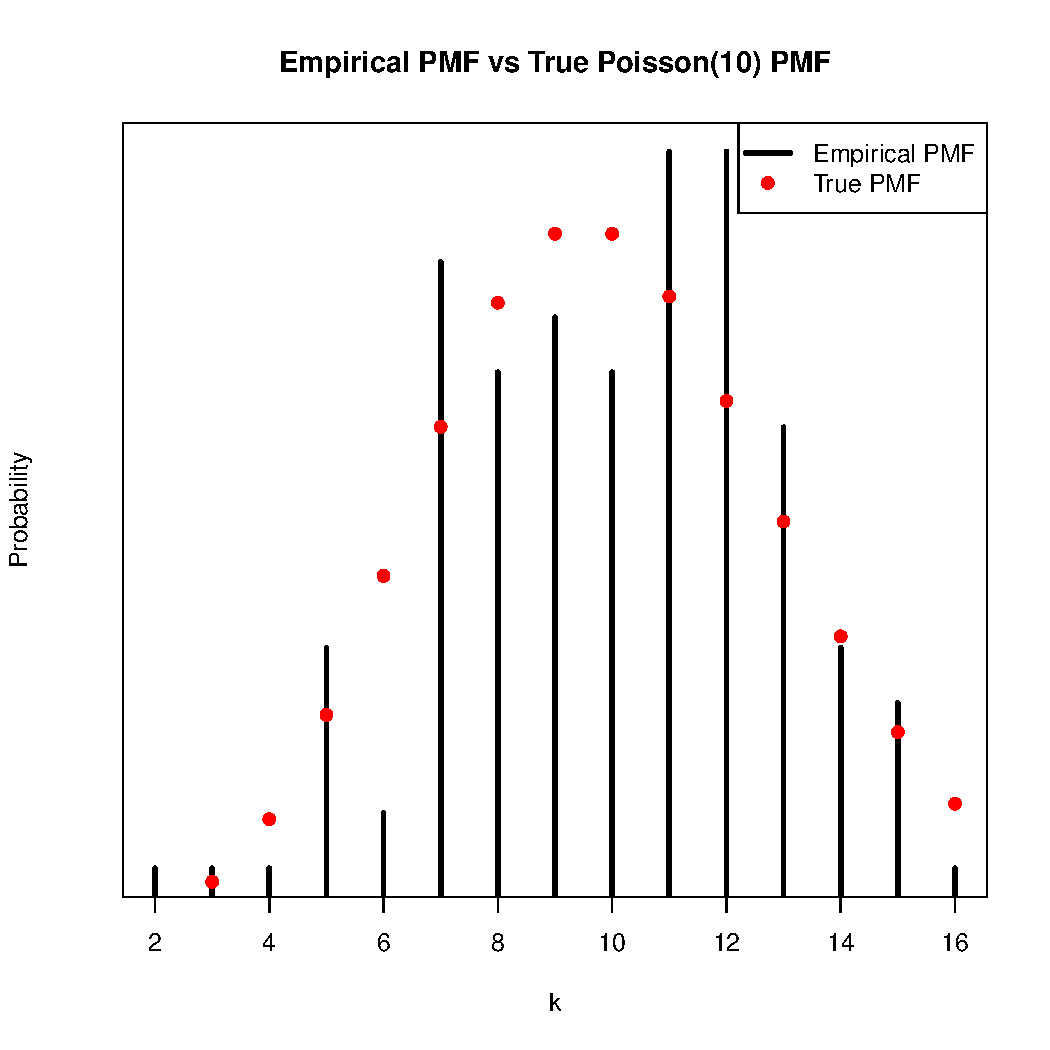
\includegraphics[width=\maxwidth]{figure/unnamed-chunk-2-1} 
\begin{kframe}\begin{alltt}
\hldef{emp_cdf} \hlkwb{<-} \hlkwd{ecdf}\hldef{(x)}
\hlkwd{plot}\hldef{(emp_cdf,}
     \hlkwc{main} \hldef{=} \hlsng{"Empirical CDF vs True Poisson(10) CDF"}\hldef{,}
     \hlkwc{xlab} \hldef{=} \hlsng{"x"}\hldef{,}
     \hlkwc{ylab} \hldef{=} \hlsng{"F(x)"}\hldef{)}
\hlkwd{curve}\hldef{(}\hlkwd{ppois}\hldef{(x,} \hlnum{10}\hldef{),}
      \hlkwc{col} \hldef{=} \hlsng{"red"}\hldef{,}
      \hlkwc{lwd} \hldef{=} \hlnum{2}\hldef{,}
      \hlkwc{add} \hldef{=} \hlnum{TRUE}\hldef{)}
\hlkwd{legend}\hldef{(}\hlsng{"bottomright"}\hldef{,}
       \hlkwc{legend} \hldef{=} \hlkwd{c}\hldef{(}\hlsng{"Empirical CDF"}\hldef{,} \hlsng{"True CDF"}\hldef{),}
       \hlkwc{lwd} \hldef{=} \hlnum{2}\hldef{,}
       \hlkwc{col} \hldef{=} \hlkwd{c}\hldef{(}\hlsng{"black"}\hldef{,} \hlsng{"red"}\hldef{))}
\end{alltt}
\end{kframe}
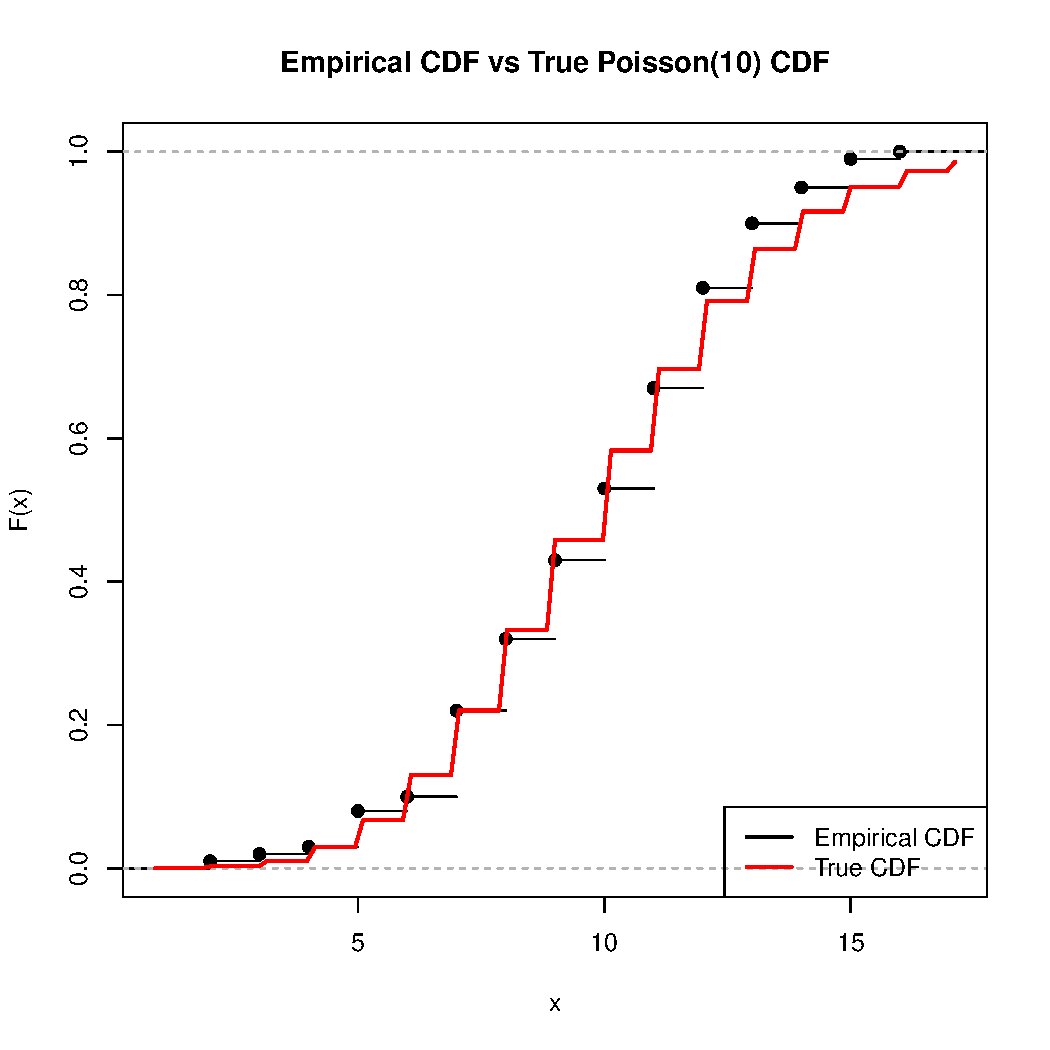
\includegraphics[width=\maxwidth]{figure/unnamed-chunk-2-2} 
\end{knitrout}





\end{document}      









